\documentclass[aspectratio = 169, 14pt]{article}
\date{}
\usepackage{graphicx}
\usepackage[spanish]{babel}
\begin{document}
\begin{titlepage}
\centering
{\bfseries\LARGE Universidad de La Habana}
\vspace{1cm}\\
{\scshape\Large Facultad de Matemática y Computación \par}
\vspace{2cm}
{\scshape\Huge\textit {MOOGLE!} \par}
\vspace{1cm}
{\itshape\Large Proyecto de Programación \par}
\vspace{4cm}
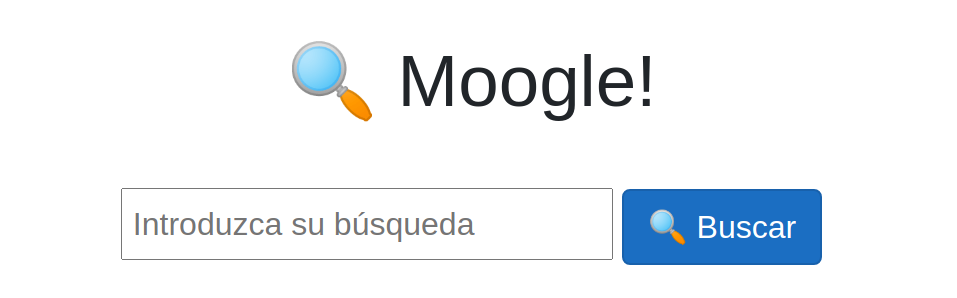
\includegraphics[width=15cm, height=4cm]{moogle.png}
\vfill
{\Large John García Muñoz C-113 \par}
{\Large Curso 2023 \par}
\end{titlepage}
\pagestyle{headings}
\parskip 3em
\begin{center}
\end{center}
\begin{flushleft}
\begin{Huge}
Funcionamiento de MOOGLE!
\end{Huge}
\setcounter{secnumdepth}{1}
\section{•Descripción}

\end{flushleft}
\begin{Large}
Moogle! es un buscador local de texto que
utiliza el modelo vectorial TF-IDF en aras de
obtener una mejora importante de eficacia y
rapidez. Se basa en la idea de crear una base
de datos con los documentos en los que se
quiere trabajar, evaluar la similaridad entre el
contenido de estos y la búsqueda realizada por
el usuario, ordenar los documentos por este
coeficiente, hacerle una sugerencia al usuario
previendo posibles errores ortográficos o de otro tipo
y finalmente mostrarle en pantalla los
documentos coincidentes ordenados, más una
frase contenida en este donde puede
encontrarse su búsqueda o algo relacionado
con esta.

\end{Large}

\section{•Funcionalidad}
\begin{Large}

- El programa cuenta con una clase
Vocabulary, en la cual se encuentran
implementados los métodos que dan forma a
la base de datos. Primeramente el método
ConvertToString() convertirá a cada
documento en texto y el método
ConvertToWorlds separará este en un array de
palabras, eliminando signos de puntuación.
Luego estos son utilizados por
GenerateMatrix(), que genera una matriz(un
array de diccionarios concretamente) en la
cual cada elemento es un diccionario
representante de un documento de texto. De
tal forma cada elemento de esta matriz es
representado como una palabra del respectivo
documento y su TF.

-La clase Moogle contiene la parte funcional
del proyecto. Primero se convierte a palabras
la query del usuario análogamente a como se
hizo con los documentos. Luego se crea un
vector que será un diccionario con los pares
palabra-IDF. A través del método vectorQuery(),
se determina un vector que contiene los pares
palabra - (TF-IDF), para luego con el método
documentsImportancy() obtener un nuevo y
último diccionario con los pares índice de
documento en la matriz - relevancia del
documento, esta se halla mediante la
multiplicación de cada vector
documento (de la matriz, formado por pares
palabra-(TF-IDF)) por el vector query, y luego
se divide este resultado por el producto de las
normas del vector documento y del vector
query mencionados. Este es el coeficiente de
similaridad que se asigna al score al
instanciar un objeto SearchItem(). Luego se
ordenan estos objetos en el array SearchItem[]
por ese score mediante el método Sort().
(Entiéndase por norma de un vector, su
concepto algebraico, que consiste en la raíz
cuadrada de la suma de sus componentes y el
score sería el coseno del ángulo entre dos
vectores).

\begin{displaymath}
SimCos(d_{(d)},q)=\frac{\displaystyle\sum_{n=1}(P_{(n,d)}\times P_{(n,q)})}{\sqrt{\displaystyle\sum_{n=1}(P_{(n,d)})^2 \times \displaystyle\sum_{n=1}(P_{(n,q)})^2}}
\end{displaymath}

-La sugerencia la fabrica el método
WordsDistance de la clase Distance, que se
encarga de comparar las palabras de la query
con las de los documentos mediante la
distancia de Levenshtein.
La distancia de Levenshtein, distancia de
edición o distancia entre palabras es el
número mínimo de operaciones requeridas
para transformar una cadena de caracteres en
otra. Se entiende por operación, bien una
inserción, eliminación o la sustitución de un
carácter. Por ejemplo, la distancia de
Levenshtein entre 'casa' y 'calle' es de 3
porque se necesitan al menos tres ediciones
elementales para convertir uno en el otro.\\
- El Snippet se obtiene mediante la clase de
mismo nombre, con el método GetSnippet().
Su función es recorrer el documento y devolver
la primera ocurrencia de la palabra más
importante de la query en ese documento.

\section{Ejecutando MOOGLE!}
Debe colocar los documentos en los que quiere desarrollar la búsqueda, en la carpeta
"Content", en formato ".txt".  

-Este proyecto está desarrollado para la versión objetivo de .NET Core 6.0. Para ejecutarlo debe ir a la ruta en la que está ubicada el proyecto y ejecutar en la terminal de Linux:

\begin{flushleft}
```bash\newline
make dev
```

- Si está en Windows, debe poder hacer lo mismo desde la terminal del WSL (Windows Subsystem for Linux), en caso contrario puede ejecutar:

```bash\newline
dotnet watch run --project MoogleServer
```

- También puede ejecutar el archivo Script.sh dentro de la carpeta Script y usar el comando "run".

\end{flushleft}
\section{•Consideraciones}
-Este programa ha sido desarrollado para
buscar en documentos en español, y no se
asegura su correcto funcionamiento en otro
idioma.\\
\newline
-La rapidez de este programa depende
necesariamente del número de documentos y
su tamaño. Su rendimiento se
verá necesariamente afectado para un número demasiado
grande de documentos extensos.
\end{Large}

\end{document}
